\chapter{Analyse comparative des  performances}
Dans cette partie, nous analysons les résultats et performances des différentes méthodes et optimisations implémentées.

Pour cela, nous avons lancé des séries de tests avec 100 itérations et avec des nombres particules différents. Nous avons donc mesuré et sommé le temps concerné pour chaque itération afin d'effectuer une moyenne pour chaque nombre de particules. Pour chaque méthode, les paramètres physiques seront les mêmes. Pour les versions parallélisées, le nombre de threads utilisés est fixé à $4$.

\section{Construction de l'arbre}

Les tests de parallélisation de notre algorithme de construction du $quadtree$ ont montré qu'il n'est pas parallélisable. En effet,  effectuer les insertions en parallèle engendre des erreurs lors  des calculs de force par l'utilisation de cet arbre, qui font diverger les particules. Cela pourrait s'expliquer par le fait que les insertions de particules sont dépendantes les unes des autres et ne peuvent donc être effectuéss en parallèle au risque de fausser les calculs. Ainsi, pour pouvoir le paralléliser, il est nécessaire de modifier au préalable le fonctionnement de l'algorithme d'insertion.

\begin{center}
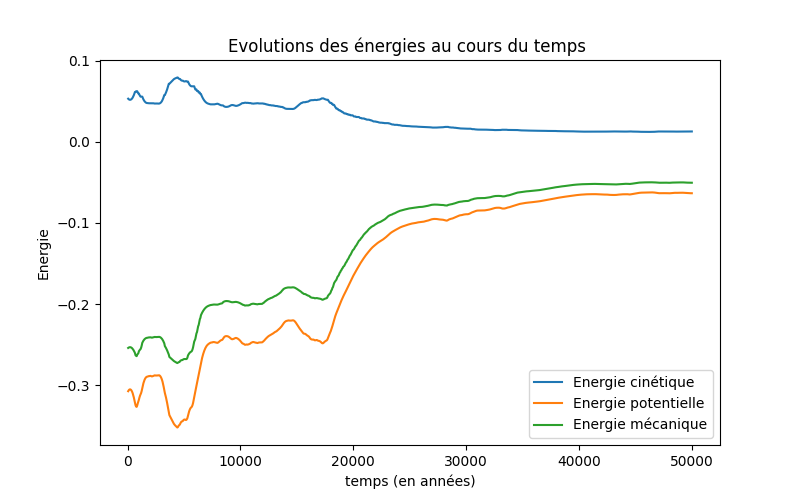
\includegraphics[scale=0.6]{./resultats/Energy_tree.png}
\captionsetup{hypcap=false}
\captionof{figure}{Bilan énergétique pour la parallélisation de la construction de l'arbre}
\label{fig11}
\end{center}

On peut voir sur la figure $7.1$ que ces erreurs se traduisent simplement par une non conservation de l'énergie mécanique au cours du temps, montrant ainsi que la parallélisation de la construction de l'arbre n'est pas intéressante.

\section{Comparaisons des méthodes}

\begin{minipage}[c]{.46\linewidth}
     \begin{center}
             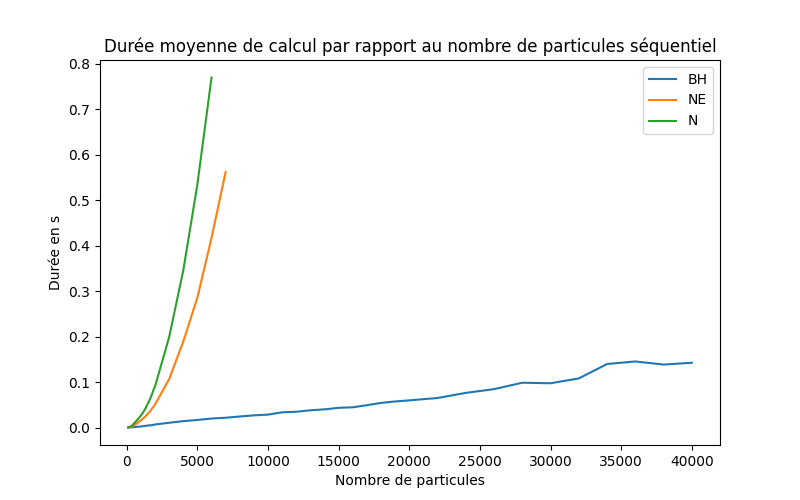
\includegraphics[width=9.5cm]{./resultats/method_comparison_seq.png}
         \end{center}
   \end{minipage} \hfill
   \begin{minipage}[c]{.46\linewidth}
    \begin{center}
     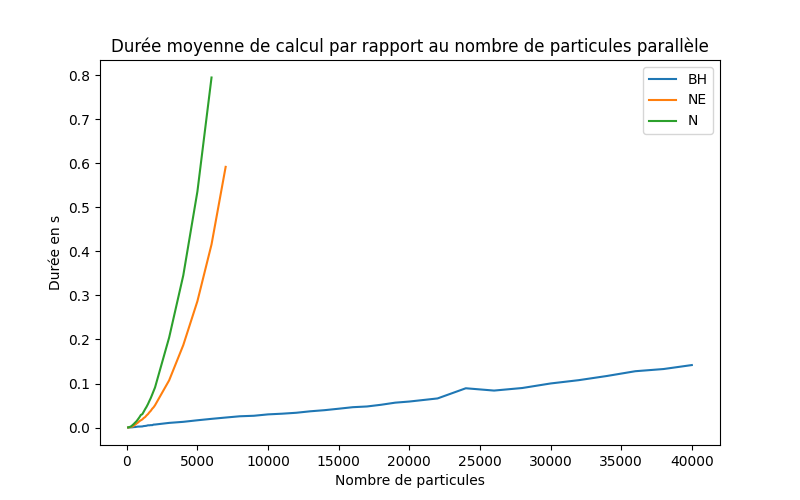
\includegraphics[width=9.5cm]{./resultats/method_comparison_par.png}
        \end{center}
 \end{minipage}
 
 \begin{center}
 \captionsetup{hypcap=false}
 \captionof{figure}{Durée moyenne en fonction du nombre de 
 particule}
\label{fig12}
 \end{center}

\par Les résultats confirment la théorie. Il est clair que les méthodes brutes ont une complexité en $O(N^2)$ alors que l'algorithme de Barnes-Hut a une complexité bien inférieure en $O(Nlog(N))$.
On peut également confirmer que l'algorithme naïf optimisé a une meilleure complexité que la version naïve.
De plus, on peut déjà remarquer que l'ordre de grandeur des durée est plus petit pour les versions parallèles.
 
\section{Séquentiel et parallèle}

\subsection{Algorithme de Barnes-Hut}
\begin{center}
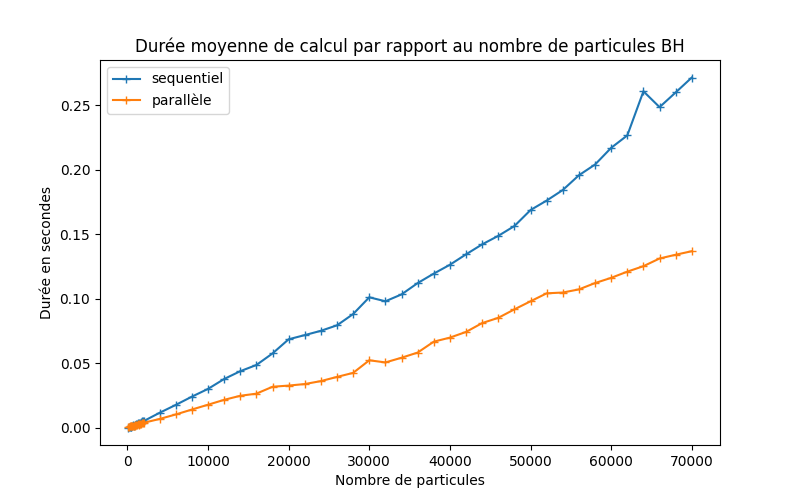
\includegraphics[scale=0.6]{./resultats/comparison_BH.png}
\captionsetup{hypcap=false}
\captionof{figure}{Résultats pour l'algorithme de Barnes-Hut}
\label{fig13}
\end{center}

On peut voir sur la figure que globalement la parallélisation améliore de manière conséquente l'efficacité des calculs. En effet, la version parallélisée est $1.7$ fois plus rapide que la version séquentielle. Dans les deux cas la complexité est en $O(log(N))$

\subsection{Naïve optimisée}
\begin{center}
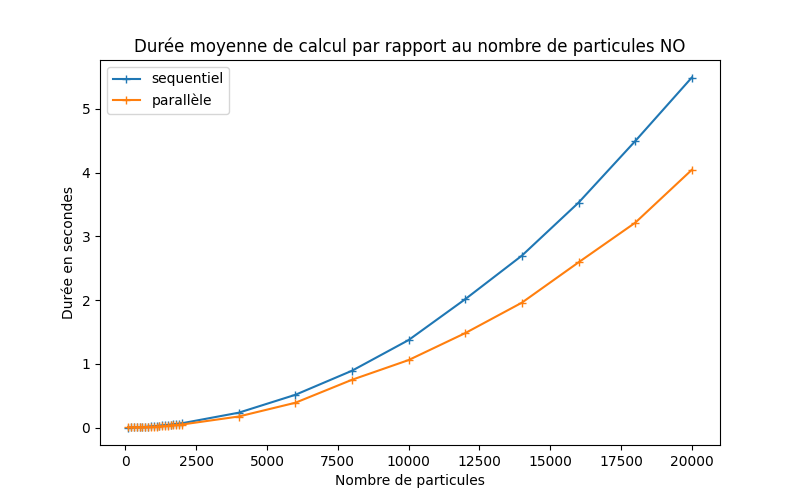
\includegraphics[scale=0.6]{./resultats/comparison_NO.png}
\captionsetup{hypcap=false}
\captionof{figure}{Résultats pour l'algorithme naïf optimisé}
\label{fig14}
\end{center}


Les résultats montrent clairement que la parallélisation est efficace et améliore la complexité de l'algorithme.
En effet, la parallélisation rend les calculs $1.4$ fois plus rapide, ce qui est déjà intéressant. Cependant, la parallélisation ne modifie pas la tendance globale de la complexité.

\subsection{Naïve}
\begin{center}
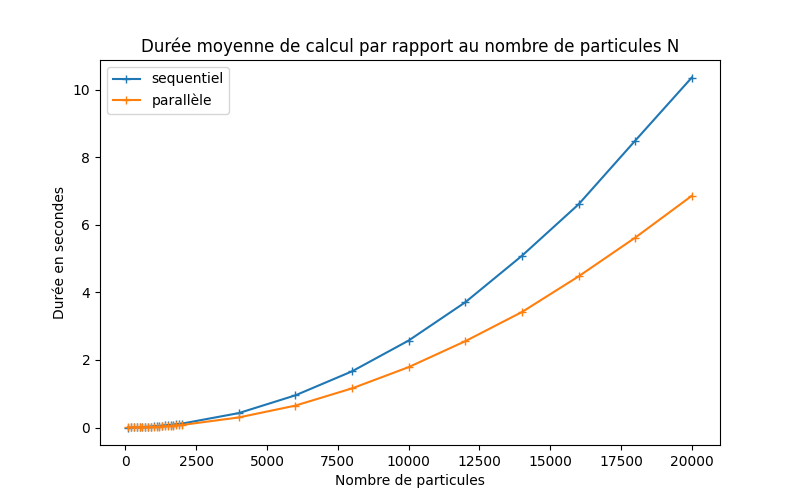
\includegraphics[scale=0.6]{./resultats/comparison_N.png}
\captionsetup{hypcap=false}
\captionof{figure}{Résultats pour l'algorithme naïf }
\label{fig15}
\end{center}


De nouveau, la parallélisation améliore les performances de l'algorithme ce qui est plutôt logique étant l'implémentation des calculs. Ainsi, la version parallélisée de la méthode est $1.5$ fois plus rapide que la version séquentielle.

\vspace{2mm}


Les résultats obtenus dans cette partie ont permis de vérifier les résultats théoriques par rapport aux performances des algorithme: l'algorithme de Barnes-Hut est bien plus performant que les autres. De plus, ils ont également montré que la parallélisation permet bel et bien d'optimiser les calculs à conditions de respecter les conditions de parallélisation. En moyenne, le gain de vitesse avec $4$ threads est d'environ $1.53$ ce qui est déjà plutôt élevé. Mais, il serait intéressant d'examiner d'autres possibles optimisations telle que l'augmentation du nombre de thread ou l'équilibre de charges entre les threads.